\documentclass[12pt]{article}
\usepackage{fullpage}
\subsectionfont{\fontfamily{phv}\fontsize{13pt}{13pt}\selectfont}
%\newcommand{\var}[1]{\mathit{#1}}
\usepackage[margin=2cm]{geometry}
\usepackage{amsmath}
\usepackage{graphicx}
\usepackage{listings}
\begin{document}
\begin{titlepage}
\newcommand{\HRule}{\rule{\linewidth}{0.5mm}} % Defines a new command for the horizontal lines, change thickness here
\center % Center everything on the page
%----------------------------------------------------------------------------------------
% HEADING SECTIONS
%----------------------------------------------------------------------------------------
\HRule \\[0.4cm]
{ \huge \bfseries Phase 3}\\[0.4cm] % Title of your document
\HRule \\[1.5cm]
\begin{minipage}{0.4\textwidth}
\begin{center} \large
Programming on the Web\\
CSC309H1, Winter 2015\\
\today
\end{center}
\end{minipage}
\vfill % Fill the rest of the page with whitespace
Cody Rosevear, c3roseve\\
999499332\\
\\
Denis Marchin, g3dmarch\\
999061009\\
\\
Farzad Hemmati, c3hemmat\\
999964953\\
\\
Akira Kakkar, g3fol\\
999825541\\
\\
\end{titlepage}
\newpage
\section*{Description}
\begin{enumerate}

\item[0.]

\textbf{URL}
http://104.236.231.174/

\textbf{Phase3 Code Snapshot}
https://mega.co.nz/#!EoMWhYoJ!k3MZ6tYcm-0HXnZOH4bv7oAG-jG89aZ3ozhByB2r1U8

\textbf{Summary Of Changes}

-Revised the feature and functionality section to be more descriptive of the user experience.

-Revised the software architecture section by adding more detail.

-Altered the project milestones section in light of current developments

-Added the justification of using MySQL

-Not testing real Paypal payments

-Validating code styling

-Employing more unit testing

-Testing in multiple web browsers

-Using Netbean’s XDebug

-Beta website deployment phase


\item[1.] Key Feature and Functionality Specification

\textbf{Homepage}

Features:
-Login button

-Register button

-Browse button

-Create button

Description: The user should be able to register, login, and reach the contact form from here.
Trying to create a project before the ser logs in should result in a redirect to the login page.
The user should, however, be able to browse projects, and only need to login in if they are going to fund it.

\textbf{Register Page}
Features:
-Email box

-Password box

-Re-enter password box

Description:
The user should be able to register via the given form.
Blank fields and emails without proper format should result in prompts to the user to correct these issues.
Some form of spam filtering should be present.
Once the form is submitted, the user should be redirected to the page they came from.

\textbf{Create profile page}

Features:
-Name box

-Email box

-Location box

-Image upload section

-Bio text area

-Password box

Description:
Here, the user should be able to edit any aspect of their profile which they see fit, and which is not related to their activity
on the website (such as reputation score, project lists etc...)
\textbf{Profile page}

Features:
-Profile picture

-Name

-Reputation score as funder and as initiator

-Initiated projects list

-Funded projects list

-Bio

-Location

-Date joined

-Recent Activity section

Description:
The profile should contain all of the basic public information for a given user. The name, location, biography should all be
alterable by the user.

The date joined, and reputation score are not alterable by the user, but determined automatically.
The reputation score will be a numeric value computed by combining all of the ratings for projects initiated by the given user with 
the number of likes their comments have recieved. In this way, a person's reputation is determined by their behaviour as both an initiator
and as a broader member of the community.

The page should also contain a feed, which displays a user's most recent activity, in the form of comments made on projects, ratings of projects,
likes of other community member's comments.

Moreover, there should also be a list of the projects initiated by the user, as well as a list of those to which the user has made contributions.

\textbf{Browse projects page}

Features:
-Search bar

-Category button to filter by project categories (within a user's communities)

-Project info box

Description:
The use should be able to filter out the projects within their community according to the pre-specified cateogires provided.
Moreover, the user should be able to enter a search term, and all of those projects associated with the term, 
and which are posted within communities
that the given user is a member off, should be filtered and shown to the user.
Each of the projects shown should display some basic information about the project, such as the title, the funding goal, and location.

\textbf{Create project page}

Features:
-Project name box

-Funding goal box

-Description box

-Pitch video (maybe)

-Funding perks box

-Project initiator  box

Description:
As the name suggests, this page is to allow users to provide the details of their project for the project info page.

\textbf{Project page}

-Project video and or image

-Creator name

-Project location

-Funding goal

-Current funding amount

-Fund button

-Project Review section (to comment on and rate projects)

Description:
This is the online pitch that other community members see when deciding to fund a project.
It should include a video or representative image of the project as well as a written description detailing the 
project and its founders.
Other users within the community should be able to rate the project (on a 5 point scale), as well as leace comments/reviews
concerning the product. The funding funding page should be accessible from this point, and all of the information pertaining
to the funding goal, how much they currently have, and how much is left to fund should be present.
\textbf{Fund page}

-Funding amount entry box

-Payment method selection box

Description:
Users should be able to enter their payment information details as well as the amount of money they want to donate to
the given project.
It should redirect the user back to the project from whence they came upon completetion of the payment process.

\textbf{Admin page}

Features:
-Total number of projects

-Total number of projects funded

-Average time to reach a funding goal

Description:
The admin page will provide the administrator with the capacity to select for viewing a number of important pre-specified statisitics.
These pre-specified statisticas will include those in the feature list, as well as any additional decided upon as development progresses.


\begin{figure}[ht!]
\centering
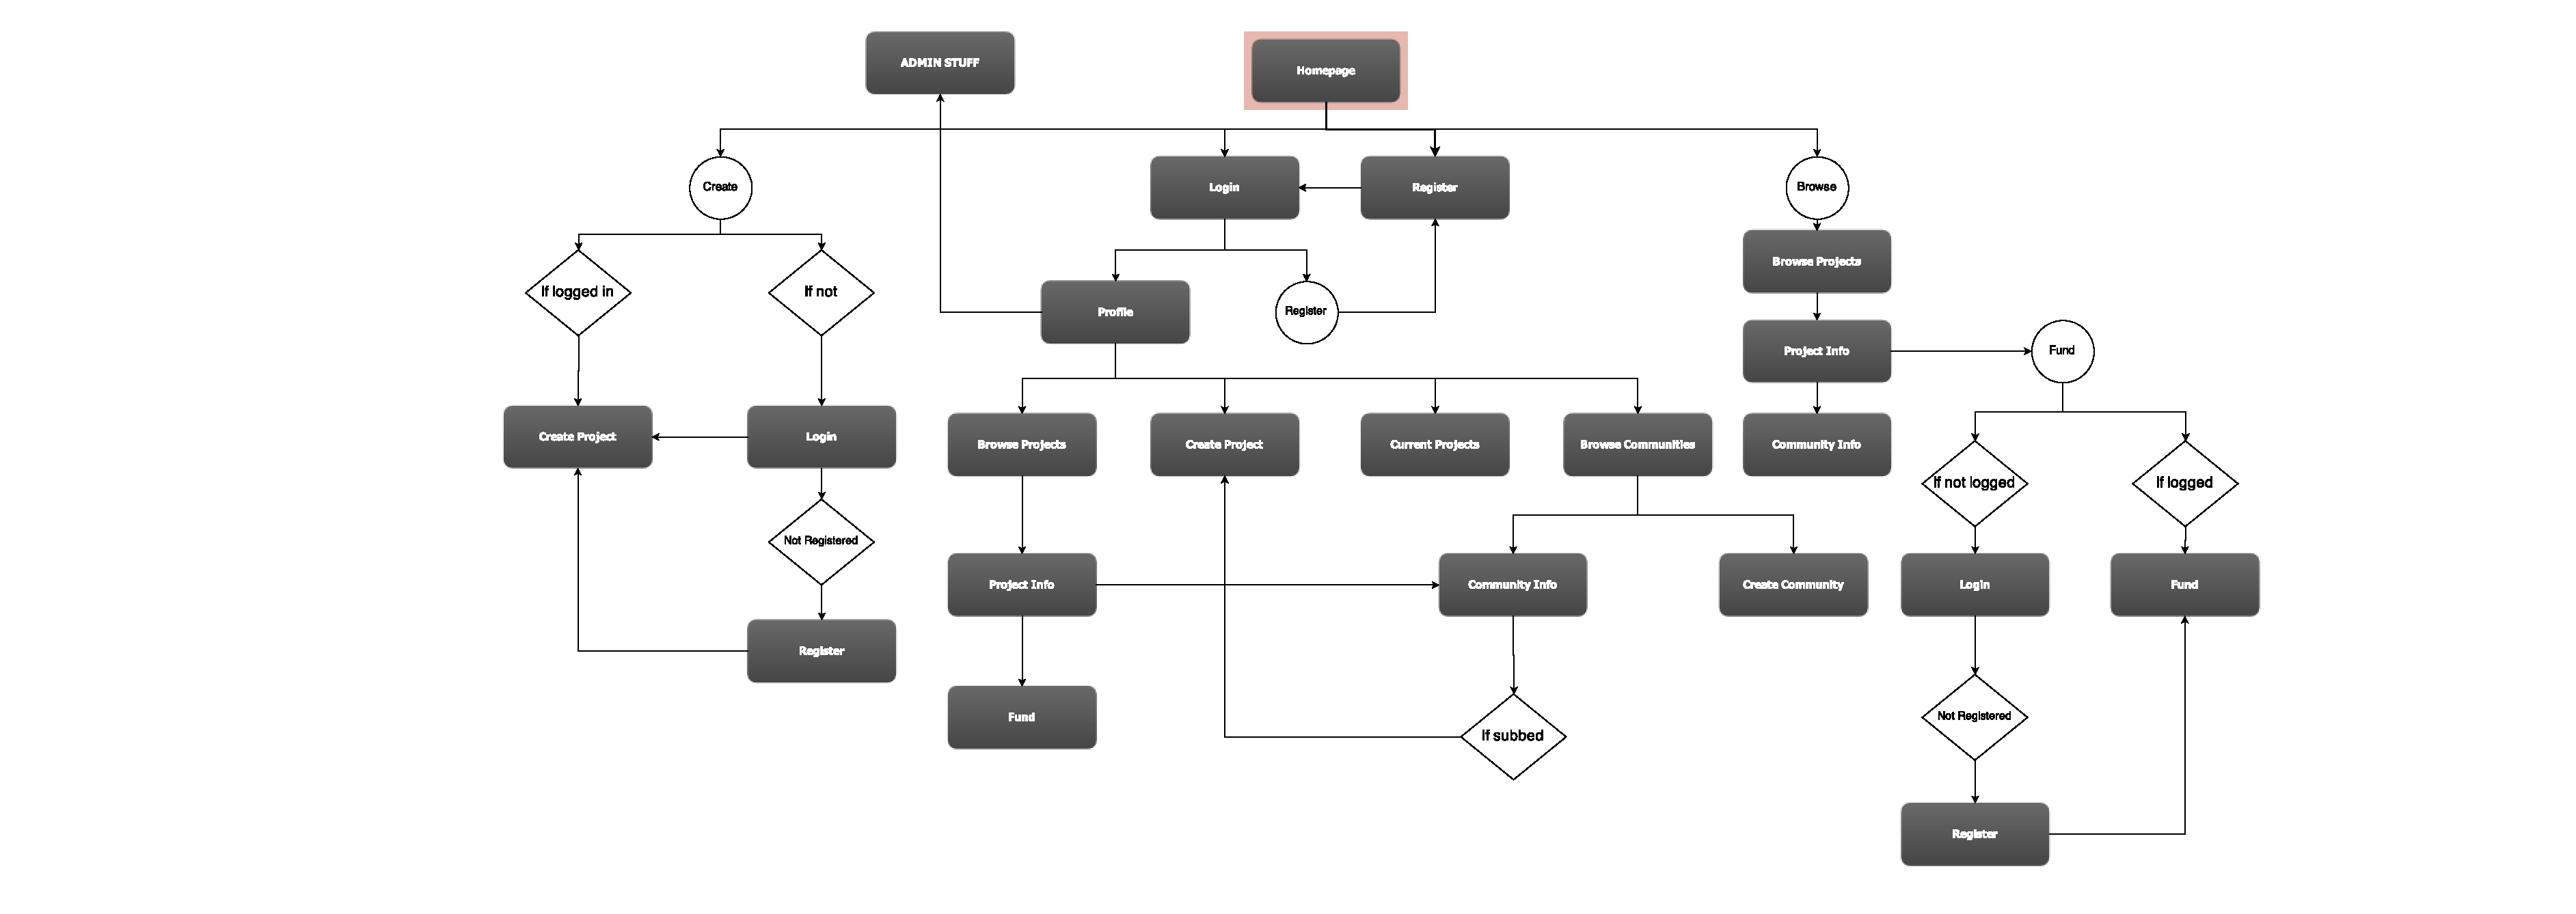
\includegraphics[width=200mm]{flowchart.pdf}
\caption{Website Flowchart \label{overflow}}
\end{figure}


\item[2.] Project Plan

\textbf{General protocol}

Communication:Weekly meetings will occur on wednesday's before class to discuss any issues related to development and write the weekly report. Moreover, Skype and Facebook will serve as methods of contact for resolving any immediate issues.

Team Roles: These will be contingent on the phase of development, and assigned for the given week at each weekly meeting. To be decided: We may segregate the team into front-end and back-end specializations.

Problem resolution: All decisions are made democratically by vote.

Hosting of Source: GitHub

\textbf{Milestones}

Note 1: The following schedule is ordered according to the perceived dependencies of the various features of the website. First the raw skeletons, then the database underlying all of the website information, followed by suitable integration between the database and web pages so that they display all of their content properly. Then, the more dynamic functionality is built weekly on top of this static base. 

Week1: Page skeletons, links, and basic styling

Week2: Central Database design and query development for all pages that use said database.

Week3: Project/Community/Profile page information is integrated with the database such that the pages display accurately.

Week4: Search functionality for all types of pages is operational.

Week5: Additional project and profile page development

Week6: Payment System and Payment System

Week7: Admin Analytics

Week8: Additional Debuggging and Development Overflow

\item[3.] Software Architecture and High-level Design
\begin{figure}[ht!]
\centering
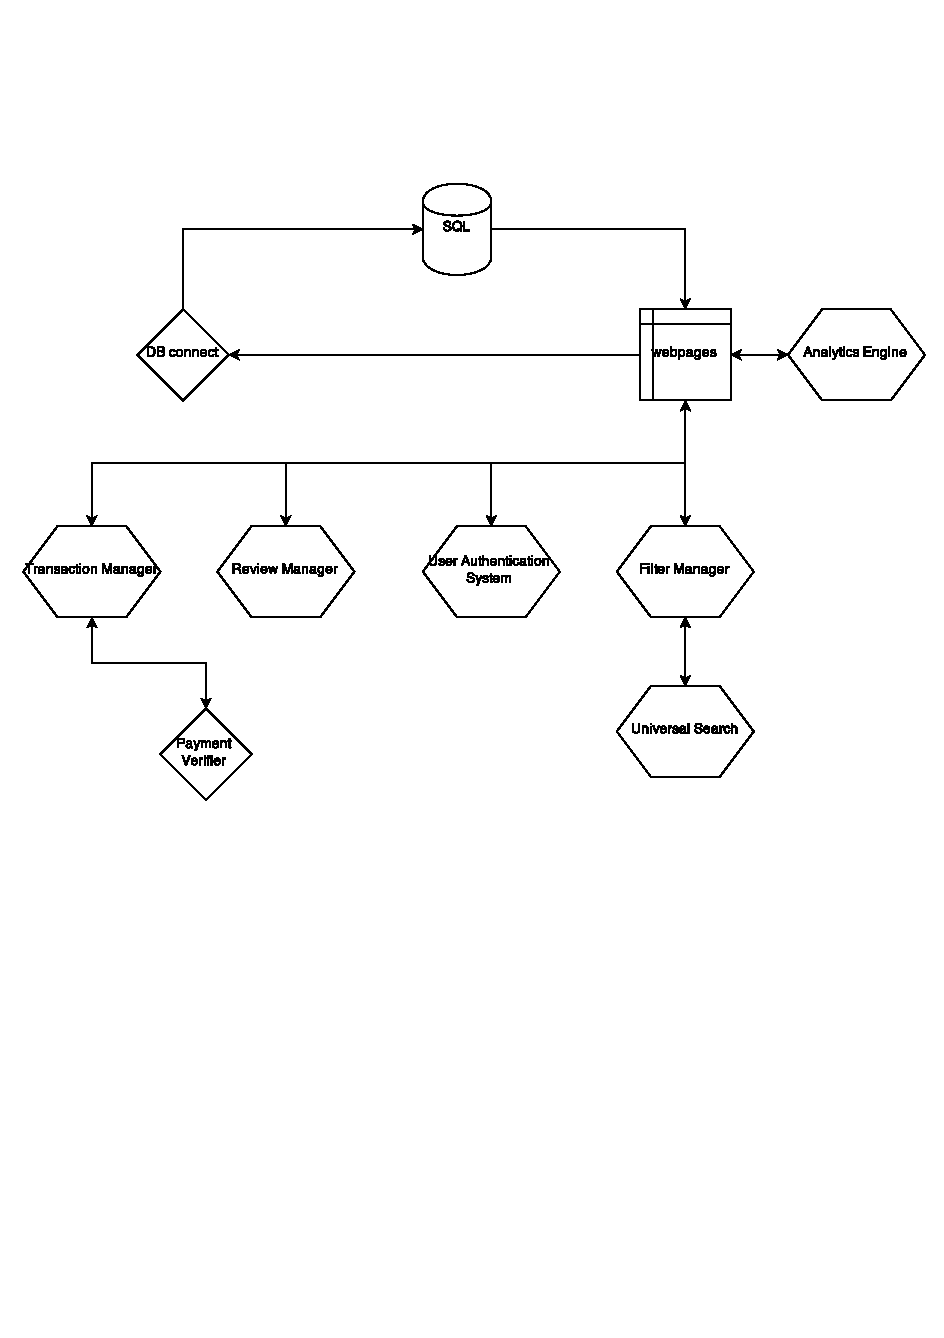
\includegraphics[width=150mm]{swag.pdf}
\caption{Software Components \label{overflow}}
\end{figure}

We are using PHP as our server-side language. For our front-end we will be using Javascript and JQuery. For our html and css design, we are going to be using bootstrap3.

We will have a central MySql database which keeps track of all the data associated with each of the various webpages. This will be the central repository from which all of the information webpages will request information when displaying webpages to users. It will also serve as the storehouse for transaction logging.

We will also have a database connector module that will be used by all of the webpages, so as to avoid code duplication.

All of the individual manager components are subsets of the functionality of the webpages themselves, and are therefore connected to the central database inasmuch as the webpages are connected to it.

The filter manager is the core software componenet that subserves all of the search functionality of the browse pages (both project and community). The filter manager will, in effect, be a more specialized instance of the code utilized for universal search throughout the website.

The transaction manager will require interaction with the central repository, since transactions will be logged in addition to processed. It will, of course, have a subfunction that verifies the payement by interacting with a third party (Paypal/credit card company).

The review manager provides the functionality to each project page which allows for funders to comment on projects as well as the reviews of other funders. It will need to be decomposed into both a rating system as well as a comment system.

The admin analytics componentt subserves the unique features of the admin view. It interacts with the central database, using the data stored there to compute statistics. This will need to be further decomposed into various functions that compute said statistics.

In terms of errors, we will display the corresponding error to the user. If the database is down and a user tries to access it, we will report to the user that database servers are down. All of this is already implemented for phase 3.


Finally, the user authentication system will be utilized wherever any kind of authentication is necessary. Since the process should generally be the same irrespective of the reason for authentication, it can be modularized.


\item[4.] Information Representation\\
User(\underline{userId} name, email, dob, password)\\
Transaction(\underline{user}, \underline{project}, \underline{date}, amount)\\
Communities(\underline{cId}, \underline{project})\\
Project(\underline{pId}, name, description, date, creator, totalAmount, community)\\
Review(\underline{project}, \underline{rate})\\
MemberOf(\underline{community}, \underline{user})\\
\\
Project(creator) \subseteq User(userId)\\
Transaction(user) \subseteq User(userId)\\
MemberOf(user) \subseteq User(userId)\\
Review(project) \subseteq Project(pId)\\
Transaction(project) \subseteq Project(pId)\\
Community(project) \subseteq Project(pId)\\
MemberOf(community) \subseteq Communities(cId)\\
Project(community) \subseteq Communities(cId)\\

MySQL is chosen because most of our group members were familiar with the technology.
Also, it goes well with php and low cost of ownership.
 

\item[5.] Test Strategy and Test Plan

Just as project initiators on this site will test their ideas and creations, we have been testing the website. Hard staff responsibilities are assigned on a weekly basis. All team members are responsible for testing the website. Website builders are expected to do some level of testing as they create a feature. GitHub is used to store the group’s file assets. When a feature has been sufficiently tested, the corresponding files are committed to the shared repository. Heavy testing of the feature from as many angles as possible will be completed nearer the end of the project phase, which is nearing. When all pages and features have been created, the testing will go into beta. During the beta phase of development, the team will shift their focus from content creating, to content testing. Basic testing is done in a timely manner, and before starting new feature additions. Record keeping of testing takes place. Untested, and therefor possibly broken additions, should be marked as such in the commit message. Features that have been tested to work properly will also be marked as such in the commit message. At our weekly meetings, team members are expected to give a report update on what testing they have completed that week, and we will distribute the new testing tasks.\\
The development team is employing an array of test strategies to ensure a properly functioning website. The user interface needs testing. We want the website to feel intuitive and easy to use. We do not want to discourage users by having a steep learning curve. As the webpages are built, the layout and navigation will be tested for user friendliness. The website will be tested in the most popular web browser programs: Internet Explorer, Firefox, Safari, and Chrome. Layout may be displayed differently upon different browsers, and we want to ensure an appealing style across all browsers the user may use. Near the end of the project phase, we will illicit our peers to test the website for ease of use. The major testing is for the databases. We are using phpMyAdmin for database management. Queries are tested for correctness. We ensure data is received and is outputted correctly. Error messages are coded-in to alert testers and users of foreseeable problems, such as not being connect to the server. Security is an extremely important element to test. We are storing sensitive information in our database, such as passwords and emails, and have a responsibility to protect the data of our users. The databases are currently populated with dummy data in order to simulate the site being operational, with many users, communities, projects, and their interactions. Common security flaws are assessed and tested against, such as SQL injection. Data validation is extensively tested, with test cases to guarantee only appropriate data in accepted. Unit testing will be used to test individual components to simplify the scope of problems. Examples of units tested are the header and footer, which are now incorporated on each page after being tested to work on their own. Users will be able to search for project using various categories. Unit testing will be used to test the site’s search function. Each type of search will be tested, and will use a test database to search against. Proper code layout is important for clarity and is a best practice. Having a uniform standard for the code layout is especially important when working in a multi-person group. Code is tested in a style validator such as W3C Markup Validator. Code layout will also be evaluated by the team as each member is to look over each line before the final submission. Development team members are free to use any program to write page code in, such as Sublime Text Editor. Code is encouraged to be written in an IDE with a comprehensive debugger, such as Netbeans. Code written outside of an IDE can still later be tested in one. XDebug from NetBeans IDE is used to test PHP. Using XDebug, the developer can cause pauses at breakpoints and retrieve information about the current program state, such as the values of the program variables. As the team does not have sufficient funds for professional software, we are relying on open source or free-to-use testing methods. Our webpage contains a “Contact us” option on every page, allowing users to report any problems they might encounter while using the website. Creating not only a working site, but an enticing one, through the process of thorough testing will give this site the potential for popularity.

\end{enumerate}
\end{document}
